\documentclass{beamer}
\usetheme{Singapore}
\usepackage{changepage}

%\usepackage{pstricks,pst-node,pst-tree}
\usepackage{amssymb,latexsym}
\usepackage{tikz}
\usepackage{graphicx}
\usepackage{fancyvrb}
\usepackage{hyperref}
\usepackage{fancybox}
\usepackage[listings]{tcolorbox}

\definecolor{codegreen}{rgb}{0,0.6,0}
\definecolor{codegray}{rgb}{0.5,0.5,0.5}
\definecolor{codepurple}{rgb}{0.58,0,0.82}
\definecolor{backcolour}{rgb}{0.95,0.95,0.92}

\lstdefinestyle{mystyle}{
    language=Python,
    backgroundcolor=\color{backcolour},   
    commentstyle=\color{codegreen},
    keywordstyle=\color{magenta},
    numberstyle=\tiny\color{codegray},
    stringstyle=\color{codepurple},
    basicstyle=\ttfamily\footnotesize,
    breakatwhitespace=false,         
    breaklines=true,                 
    captionpos=b,                    
    keepspaces=true,                 
    numbers=left,                    
    numbersep=5pt,                  
    showspaces=false,                
    showstringspaces=false,
    showtabs=false,                  
    tabsize=2,
    escapechar=|,
    frame=single
}

\lstset{style=mystyle}


\newcommand{\bi}{\begin{itemize}}
\newcommand{\li}{\item}
\newcommand{\ei}{\end{itemize}}
\newcommand{\Show}[1]{
\begin{center}
\shadowbox{\begin{minipage}{0.8\textwidth}
          #1
          \end{minipage}}
\end{center}
}
\newcommand{\arrow}{\ensuremath{\rightarrow}}

\newcommand{\uparr}{\ensuremath{\uparrow}}


\newcommand{\fig}[2]{\centerline{\includegraphics[width=#1\textwidth]{#2}}}

\newcommand{\bfr}[1]{\begin{frame}[fragile]\frametitle{{ #1 }}}
\newcommand{\efr}{\end{frame}}

\newcommand{\cola}{\begin{columns}\begin{column}{0.5\textwidth}}
\newcommand{\colb}{\end{column}\begin{column}{0.5\textwidth}}
\newcommand{\colc}{\end{column}\end{columns}}


\title{Algorithm Analysis}
\author{CSCI 112, Winter 2023, Lecture 1}

\begin{document}

\begin{frame}
\maketitle
\end{frame}

\bfr{Review Python}
\cola
\bi
\li Strings
\li Lists
\li Tuples
\li Dictionaries
\li Sets
\li List comprehensions
\li Functions, including {\tt lambda}
\li Classes
\li Exception handling
\li Unit tests
\ei
\colb
\bi
\li
All of these are reviewed in your textbook.
\li
Review the exercises at the end of the chapter.
\li
There are also many online Python tutorials.
\ei
\colc
\end{frame}

\bfr{Algorithm Analysis}
\end{frame}

\bfr{Algorithms}
\cola
\bi\li Classic multiply\ei
\begin{Verbatim}[frame=single]
        238
      x  13
     ------
        714      
       238 
     ------
       3094
\end{Verbatim}
\colb\pause
\bi \li Peasant multiply \ei
\begin{Verbatim}[frame=single]
    238   13   -->   238
    476    6
    952    3   -->   952
   1904    1   -->  1904
                    ----
                    3094
\end{Verbatim}                   
\colc

\end{frame}

\bfr{Programs}
\begin{lstlisting}
def classic_multiply(a, b):
    bdigits = reversed([int(x) for x in list(str(b))])
    sum = 0
    for i, digit in enumerate(bdigits):
        sum += digit * a * 10 ** i
    return sum
\end{lstlisting}
\begin{lstlisting}
def peasant_multiply(a, b):
    sum = 0
    while b > 0:
        if b % 2 == 1:
            sum += a
        a, b = a*2, b//2
    return sum  
\end{lstlisting}

Which is better?  What does that even mean?
\end{frame}
\bfr{Algorithm {\em vs} Program}
\bi
\li An {\bf algorithm} is an explicit, step-by-step procedure
for solving a problem.
\bi
\li There can be many algorithms to solve the same problem.
\li There are problems for which there exists no algorithm!
\ei
\li A {\bf program} is an explicit, step-by-step set of instructions to a computer.
\bi
\li Usually, a program is an {\bf implementation} of an 
algorithm.
\ei
\ei
\end{frame}

\bfr{Measuring runtime}
\cola
\begin{lstlisting}
a=5
b=6
c=10
for i in range(n):
   for j in range(n):
      x = i * i
      y = j * j
      z = i * j
for k in range(n):
   w = a*k + 45
   v = b*b
d = 33
\end{lstlisting}
\bi
\li We could time it.
\li That would depend on processor, {\em etc.}
\li Hard to compare this algorithm with another.
\ei
\colb
\bi
\li Better to, {\em e.g.}, count the number of assignments.
\li There are 4 assignments outside the loops.
\li There are 3 in the body of the first loop, which is done $n^2$ times.
\li There are 2 in the body of the second loop, which is done $n$ times.
\li Total number of assignments: $3n^2 + 2n^2 + 4$
\ei
\colc
\end{frame}


\bfr{Measuring runtime}

\begin{lstlisting}
a=5
b=6
c=10
for i in range(n):
   for j in range(n):
      x = i * i
      y = j * j
      z = i * j
for k in range(n):
   w = a*k + 45
   v = b*b
d = 33
\end{lstlisting}
\bi
\li
Total number of assignments: $3n^2 + 2n^2 + 4$
\li
As $n\rightarrow \infty$, this function is dominated by the $3n^2$ term.
\li
We don't care about constants, because that is just units.
\li
We say that this program is {\bf order} $n^2$, or
\[O(n^2)\]
\ei
\end{frame}
\bfr{A refresher on some basic math}
\end{frame}

\bfr{Logarithms}

\centerline{\shadowbox{\small Logarithms, by shortening the labors, doubled the life of an astronomer.}}

\hfill  \sl-- Pierre-Simon, marquis de Laplace

\cola
\begin{align*}
\log_b(a) &= c  \Leftrightarrow b^c = a\\\\
\log_b(ac) &= \log_b(a) + \log_b(c)\\
\end{align*}
\colb
\hfill 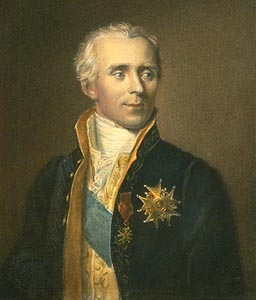
\includegraphics[width=0.5\textwidth]{laplace}
\colc
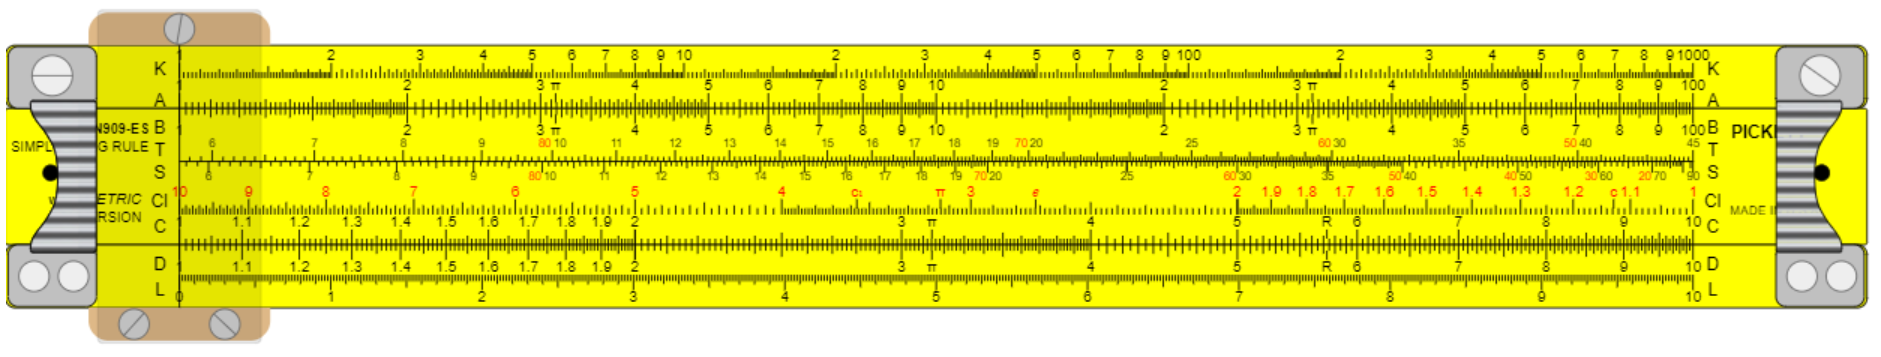
\includegraphics[width=\textwidth]{sliderule}

\centerline{\url{https://www.sliderules.org/}}
\end{frame}


\bfr{Logarithm refresher}
\[
\log_b(a) = c  \Leftrightarrow b^c = a
\]
\begin{align*}
b^{\log_b(a)} &= a\\
\log_b(ac) &= \log_b(a) + \log_b(c)\\
\log_b(a) &= \frac{\log_d(a)}{\log_d(b)} & \frac{a}{b} = \frac{a/d}{b/d}\\
\log_d(b)\log_b(a) &= \log_d(a) & \frac{b}{d}\frac{a}{b} = \frac{a}{d}\\
\log_b(a) &= \frac{1}{\log_a(b)}\\
\log_b(a) &= k\log_d(a) &
\log_{10}(1203248) &\approx 6\\
&&\log_2(1203248) &\approx 20
\end{align*}
\end{frame}

\bfr{Summation rules}

\begin{align*}
\sum_{i=m}^n c &= (n - m + 1)c 
\\\\
\sum_{i=m}^n ca_i &= c\sum_{i=m}^n a_i 
\\\\
\sum_{i=m}^n (a_i + b_i) &= \sum_{i=m}^n a_i + \sum_{i=m}^n + b_i
\end{align*}
\end{frame}


\bfr{Summation rules}

\begin{align*}
\sum_{i=m}^n a_{i+k} &= \sum_{i=m+k}^{n+k} a_{i}
\\\\
\sum_{i=m}^n a_{i}x^{i+k} &= x^k \sum_{i=m}^{n} a_{i}x^i
\\\\
\sum_{i=m}^n (a_i - a_{i-1}) &= a_n - a_{m-1}
\end{align*}

\centerline{\scriptsize
\url{https://tutorial.math.lamar.edu/classes/calci/summationnotation.aspx}
}

\centerline{\scriptsize
\url{https://www.math.brown.edu/johsilve/MA0075/SummationTutorial.html}
}

\end{frame}

\bfr{Sum of constant}

\begin{align*}
  \sum_{i=1}^n 1 &=  1+1+1\ldots+1\\&=n\\
                 \\
  \sum_{i=1}^n c &=  c+c+c\ldots+c\\&=cn\\\\
\end{align*}
\end{frame}

\bfr{Sum of $i$}
\[
\begin{array}{cccccccccc}
 & \sum_{i=1}^n i &=& 1 &+& 2 &+& \ldots  &+& n
\\
+&  \sum_{i=1}^n i  &=& n &+& n-1 &+& \ldots  &+& 1
\\
\multicolumn{10}{c}{\hrulefill}
\\
 &&=& n+1 &+& n+1 &+& \ldots  &+& n+1
  \\
 & &=& \multicolumn{3}{l}{n(n+1)}
  \\\\\\
\Rightarrow&  \sum_{i=1}^n i &=& \multicolumn{3}{l}{\frac{n(n+1)}{2}}
\end{array}
\]
\end{frame}

\bfr{Sum of $i$, another way}
\cola
\begin{align*}
\sum_{i=m}^n (a_i - a_{i-1}) &= a_n - a_{m-1}\\\\\\
  n^2 &= n^2 - 0^2
\end{align*}
\colb
\begin{align*}
  n^2&= \sum_{i=1}^n (i^2 - (i-1)^2)
  \\
  &= \sum_{i=1}^n (2i - 1)
  \\
  &= 2\sum_{i=1}^n i - \sum_{i=1}^n 1
  \\
  &= 2\sum_{i=1}^n i - n
  \\
  &\Rightarrow  \sum_{i=1}^n i = \frac{n^2+n}{2}
\end{align*}
\colc
\end{frame}

\bfr{Sum of $i$, easiest way}
\[
\sum_{i=1}^n i = \frac{n(n+1)}{2}
\]
\begin{center}
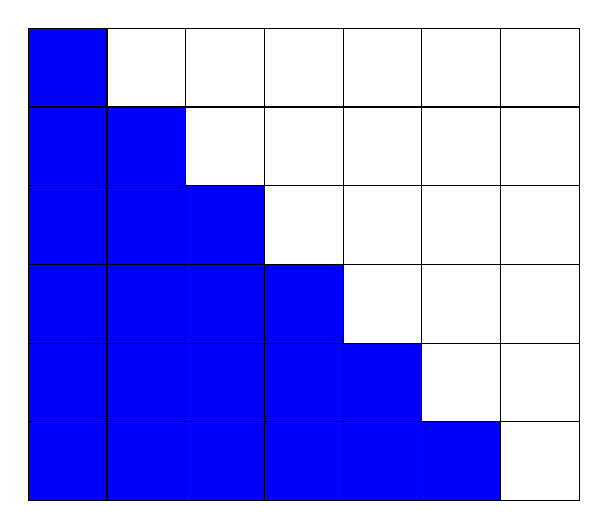
\begin{tikzpicture}
\fill[blue] (0,0) rectangle (6,1);
\fill[blue] (0,1) rectangle (5,2);
\fill[blue] (0,2) rectangle (4,3);
\fill[blue] (0,3) rectangle (3,4);
\fill[blue] (0,4) rectangle (2,5);
\fill[blue] (0,5) rectangle (1,6);
\draw[black] (0,0) grid (7,6);
\end{tikzpicture}
\end{center}

\end{frame}

\bfr{Sum of Odd Numbers}
\begin{align*}
1 + 3 + \ldots + (2n+1) &= \sum_{i=0}^n (2i+1) 
\\
&= \sum_{i=0}^n 2i + \sum_{i=0}^n 1
\\
&= 2\sum_{i=0}^n i + (n+1)
\\
&= 2n(n+1)/2 + (n+1)
\\
&= (n+1)^2
\end{align*}
\end{frame}


\bfr{Geometric Sum}
\cola
\begin{align*}
  S_n &= 
   \sum_{i=0}^n a^i\\
  &= 1 + a + a^2 + \ldots + a^n
  \\
  S_{n+1} &= (1 + a + a^2 + \ldots + a^n) + a^{n+1}
  \\
  &= S_{n} + a^{n+1}
  \\
  S_{n+1} &= 1 + (a + a^2 + \ldots + a^n + a^{n+1})
  \\
  &= 1 + a(1 + a + a^2  +  \ldots + a^n)
  \\
  &= 1 + aS_n
\end{align*}
\colb
\begin{align*}
  S_n + a^{n+1} &= 1 + aS_n
  \\
  &\Rightarrow\\
 S_n
  &= \frac{a^{n+1} - 1}{a-1}\\
  &=   \sum_{i=0}^n a^i 
\end{align*}
\colc
\end{frame}

\bfr{Geometric sum, another way}
\begin{align*}
(a-1)\sum_{i=0}^n a^i &= \sum_{i=0}^n \left(a^{i+1} -a^i\right)\\
  &= \sum_{i=1}^{n+1} \left(a^{i} - a^{i-1}\right)\\
  &= a^{n+1} - a^0\\
  &= a^{n+1} - 1\\\\
  \sum_{i=0}^n a^i &= \frac{a^{n+1} - 1}{a-1}
\end{align*}
\end{frame}

\bfr{Geometric Sum}
\begin{align*}
\sum_{i=0}^n a^i &= \frac{a^{n+1} - 1}{a-1}
\end{align*}
If $a>1$ and $n$ is large, then
\begin{align*}
a^{n+1}-1 &\approx a^{n+1}
\end{align*}
Therefore
\begin{align*}
1+a+a^2+\ldots+a^n &= \frac{a^{n+1}-1}{a-1}\\
  &\approx \left(\frac{a}{a-1}\right) a^n\\
  &= ka^n& 1<k\leq2
\end{align*}
  

\end{frame}

\bfr{Memorizing the Geometric Sum}
\begin{align*}
\sum_{i=0}^n a^i &=
1 + a + a^2 + \ldots + a^n\\
 &\approx a^n\\\\
 &= \frac{a^{n+1}}{a} \\\\
 &\approx \frac{a^{n+1} -1}{a-1}
 = 
\sum_{i=0}^n a^i
\end{align*}
\end{frame}

\bfr{Algorithm analysis}
\bi
\li We want to study the runtime of programs.  How long does it take
to solve a problem with the computer?
\li Constants don't matter, since it is just a change in units.
Two minutes or 120 seconds?  Units are arbitrary.
\li We also don't care about machine speed, programming language, etc.
A computer that is twice as fast will just add a constant
factor of $1/2$, anyway.
\ei
\end{frame}

\bfr{Algorithm analysis}
\bi
\li We are also especially interested in how well
programs scale to larger and larger problems.
If the problem is ten times bigger, will it take
ten times as long to solve?  More?  Less?
\li
This is the essence of what we want to measure.
The {\bf growth rate} of a program's execution time as the
problem gets larger.
\li
We generally measure {\bf the number of times something is done.}
This will be a positive integer independent of units.
\ei

\end{frame}

\bfr{Big O notation}
\bi
\li We assume all our functions are positive integers (they measure number
of times something is done).
\li We say that a function $f(x)$ is  Big-O   $g(x)$, 
\[ f(x) = O(g(x)) \]
if there is some constant, $C$, such that $f(x) \leq Cg(x)$
for $x$ big enough.
\li Example, let $f(x) = 3x^2 + 10x + 2$.  Then $f(x) = O(x^2)$ because
\begin{align*}
f(x) &= 
3x^2 + 10x + 2 \\
&\leq 3x^2 + 10x^2 + 2x^2 & \mbox{if }x \geq 1\\
  &= 15x^2
\end{align*}
\ei

\end{frame}
\bfr{Big O notation}
\bi
\li Note that $f(x) = 3x^2 + 10x + 2$
is also $O(x^3)$, since
\begin{align*}
f(x) &= 
3x^2 + 10x + 2 \\
&\leq 3x^3 + 10x^3 + 2x^3 & \mbox{if }x \geq 1\\
  &= 15x^3
\end{align*}
\li However, $f(x) \not = O(x)$, because,
let $C$ be any constant, then
\begin{align*}
Cx &< x^2 &\mbox{if } x > C\\
   &< 3x^2 + 10x + 2 &\mbox{if } x > max(1,C)\\
   &= f(x)
\end{align*}
\li
So it is not possible to find $C$
such that $f(x) \leq Cx$ for large $x$.
\li If $C$ is large, say $C = 10^{1000000}$,
then $f(x) \leq Cx$ for quite a few values
of $x$.  But, eventually, ...
\ei
\end{frame}

\bfr{Summing up}
\begin{align*}
f(x) &=  3x^2 + 10x + 2\\
f(x) &= O(x^3)\\
f(x) &= O(x^2)\\
f(x) &\not= O(x)\\
f(x) &\not=O(1)
\end{align*}
\bi
\li We say $O(x^2)$ is a {\bf tight} bound.
\li $O(x^3)$ is a {\bf loose} bound.
\li Generally we prefer to find bounds as tight
as possible.
\ei
\end{frame}

\bfr{Alternate method for showing Big-O}
If $f(x)$ and $g(x)$ are continuous, then
\begin{align*}
\lim_{x\rightarrow\infty} \frac{f(x)}{g(x)} &< \infty
\end{align*}
implies
\begin{align*}
f(x) = O(g(x))
\end{align*}

For example:
\begin{align*}
\lim_{x\rightarrow\infty}\frac{3x^2 + 10x + 2}{x^2} = 3
\end{align*}
And so $3x^2+10x+2 =O(x^2)$

\vfill
We can also use l'Hopital's rule!
\end{frame}

\bfr{Big O Hierarchy}
\cola
\begin{align*}
   & O(1) 
\\ & O(\log(\log(n)))
\\ & O(\log n)
\\ & O(\sqrt{n})
\\ & O(n)
\\ & O(n\log n)
\\ & O(n^2)
\\ & O(n^2\log n)
\\ & O(n^3)
\\ & O(2^n)
\\ & O(3^n)
\\ & O(n!)
\end{align*}
\colb
\bi
\li Each function is Big-O of all the functions below it.
\li No function is Big-O of any function above it.
\li   Since
log to one base is a constant multiple of log
to a different base:
\begin{align*}
\log_a n  &= O(\log_b n)
\end{align*}
for any bases $a$ and $b$.
\ei

\colc

\vfill

\centerline{\url{https://www.bigocheatsheet.com/}}
\end{frame}
\bfr{Big O Chart}
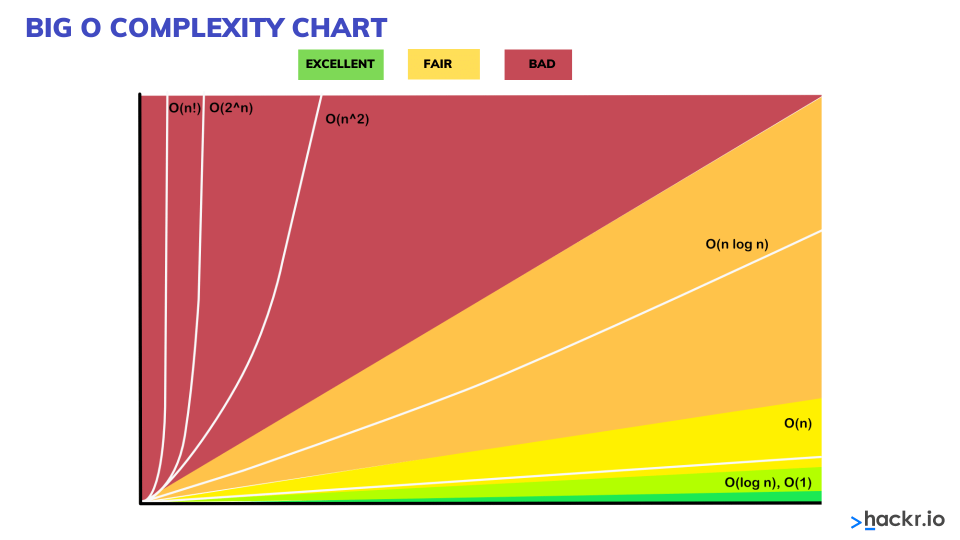
\includegraphics[width=\textwidth]{bigo}
\end{frame}


\bfr{Algorithm Analysis}
How many assignment statements are made?

\begin{lstlisting}
for i in range(n):
  x = i + f(x)
\end{lstlisting}
\pause
\begin{align*}
\sum_{i=0}^{n-1}(1 + 1) &= 
 \sum_{i=0}^{n-1}2\\
  &= 2n
\end{align*}

\bi
\li This program is $O(n)$
\ei
 
\end{frame}

\bfr{Algorithm Analysis}
How many assignment statements are made?
\begin{columns}
\begin{column}{0.4\textwidth}
\begin{lstlisting}
for i in range(n):
  for j in range(n):
    x = i + j + f(x)
\end{lstlisting}
\bi
\li This program is $O(n^2)$
\ei
\pause
\end{column}
\begin{column}{0.6\textwidth}
\begin{align*}
\sum_{i=0}^{n-1}\left(1 + \sum_{j=0}^{n-1}(1+1)\right) &= 
 \sum_{i=0}^{n-1}\left(1+ \sum_{j=0}^{n-1}2\right)
 \\
  &= 
 \sum_{i=0}^{n-1}(1+ 2n) \\
  &= 
 \sum_{i=0}^{n-1}1+ \sum_{i=0}^{n-1}2n \\
  &= 
 n+ 2\sum_{i=0}^{n-1}n \\
  &= 2n^2 + n
\end{align*}
\end{column}
\end{columns}
\end{frame}

\bfr{Visualizing nested {\tt for} loops}
\cola
\begin{lstlisting}
for i in range(n):
  for j in range(n):
    x = i + j + f(x)
\end{lstlisting}
\colb
\[O(n^2)\]
\colc

\begin{center}
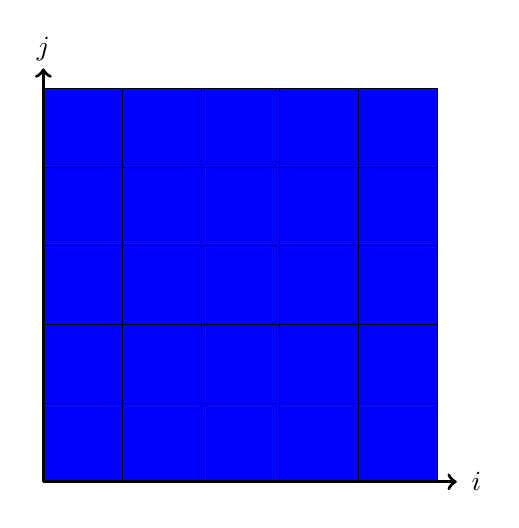
\begin{tikzpicture}
\fill[blue] (0,0) rectangle (5,5);
\draw[step=1cm,black,very thin] (0,0) grid (5,5);
\draw[very thick,->](0,0) -- (5.25,0);
\draw[very thick,->](0,0) -- (0,5.25);
\draw(5.5,0) node{$i$};
\draw(0,5.5) node{$j$};
\end{tikzpicture}
\end{center}

\end{frame}

\bfr{Algorithm Analysis}
How many assignment statements are made?
\begin{lstlisting}
for i in range(n):
  for j in range(i):
    x = x + f(x) + j
\end{lstlisting}
\pause
\begin{columns}
\begin{column}{0.6\textwidth}
\begin{align*}
\sum_{i=0}^{n-1}\left(1 + \sum_{j=0}^{i-1}(1+1)\right)
&= 
\sum_{i=0}^{n-1}\left(1 + \sum_{j=0}^{i-1}2\right)\\
&=
\sum_{i=0}^{n-1}(1 + 2i)\\
&=
\sum_{i=0}^{n-1}1 + 2\sum_{i=0}^{n-1}i\\
&= n + n(n+1)\\
&= n^2 + 2n
\end{align*}
\end{column}
\begin{column}{0.4\textwidth}
\bi
\li This function is also $O(n^2)$
\ei
\end{column}
\end{columns}
\end{frame}

\bfr{Visualizing nested {\tt for} loops}
\cola
\begin{lstlisting}
for i in range(n):
  for j in range(i):
    x = x + f(x) + j
\end{lstlisting}
\colb
\[\frac{n(n-1)}{2}=O(n^2)\]
\colc

\begin{center}
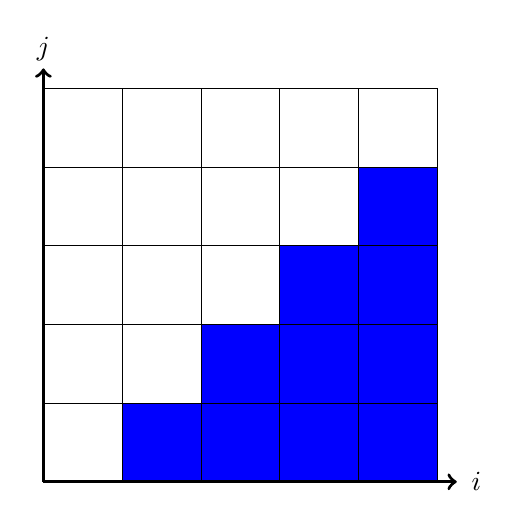
\begin{tikzpicture}
\fill[blue] (1,0) rectangle (5,1);
\fill[blue] (2,1) rectangle (5,2);
\fill[blue] (3,2) rectangle (5,3);
\fill[blue] (4,3) rectangle (5,4);
\draw[step=1cm,black,very thin] (0,0) grid (5,5);
\draw[very thick,->](0,0) -- (5.25,0);
\draw[very thick,->](0,0) -- (0,5.25);
\draw(5.5,0) node{$i$};
\draw(0,5.5) node{$j$};
\end{tikzpicture}
\end{center}

\end{frame}
\bfr{Algorithm Analysis}
How many lines does {\tt doodle} draw?
\cola
\begin{lstlisting}
def doodle(n, m):
  if n > 0:
    line(n, n, m, m)
    line(n, m, m, n)
    doodle(n-1, m)
\end{lstlisting}
\pause
\colb
\bi\li $O(n)$ \ei
\colc
\begin{align*}
f(0) &= 0\\
f(n) &= f(n-1) + 2\\
  &= (f(n-2) + 2) + 2\\
  &= ((f(n-3) + 2) + 2) + 2)\\
  &= f(n-k) + 2k \\
  &= ...\\
  &= f(n-n) + 2n\\
  &= 2n
\end{align*}
\end{frame}

\bfr{Algorithm Analysis}
How many additions does {\tt quibble} make?
\begin{lstlisting}
def quibble(n):
  if n == 0:
    return 1
  else:
    return quibble(n-1) + quibble(n-1)
\end{lstlisting}
\cola
\begin{align*}
f(0) &= 0\\
f(n) &= 2f(n-1) + 1\\
     &= 2(2f(n-2) + 1) + 1\\
     &= 2^2f(n-2) + 2 + 1\\
     &= 2^3f(n-3) + 4 + 2 + 1\\
     &= 2^4f(n-4) + 8 + 4 + 2 + 1
\end{align*}
\colb\pause
\begin{align*}
     &= 2^kf(n-k) + \sum_{i=0}^{k-1} 2^i\\
     &= 2^nf(n-n) + \sum_{i=0}^{n-1} 2^i\\
     &= 2^nf(0) + \frac{2^n-1}{2-1}\\
     &= 2^n-1 = O(2^n)
\end{align*}
\colc
\end{frame}

\bfr{Visualizing recursion}

\begin{lstlisting}
def quibble(n):
  if n == 0:
    return 1
  else:
    return quibble(n-1) + quibble(n-1)
\end{lstlisting}
\[O(2^n)\]
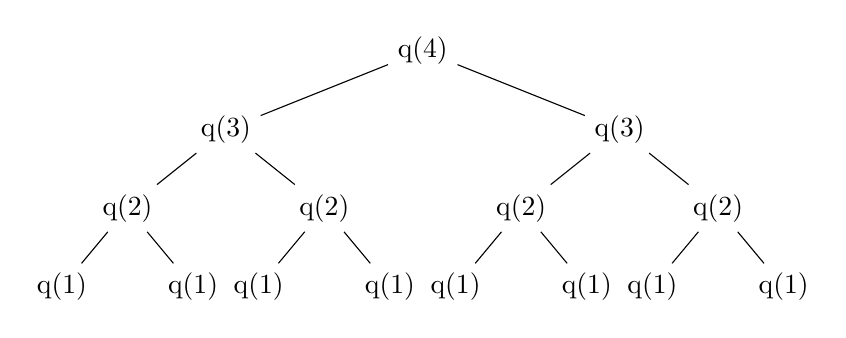
\begin{tikzpicture}[level distance=1cm,level/.style={sibling distance=5cm/(#1)}]
  \node {q(4)}
    child {node {q(3)}
      child {node {q(2)}
        child {node {q(1)}}
        child {node {q(1)}}
      }
      child {node {q(2)}
        child {node {q(1)}}
        child {node {q(1)}}
      }
      }
    child {node {q(3)}
      child {node {q(2)}
        child {node {q(1)}}
        child {node {q(1)}}
      }
      child {node {q(2)}
        child {node {q(1)}}
        child {node {q(1)}}
      }
    };
\end{tikzpicture}
\end{frame}

\bfr{Fibonacci}
\begin{lstlisting}
def fibonacci(n):
  if n < 2:
    return n
  else:
    return fibonacci(n-1) + fibonacci(n-2)
\end{lstlisting}
The mathematics is difficult, but the result is similar
to {\tt quibble}:
\[
 O(1.7)^n
\]
\end{frame}

\bfr{Visualizing Fibonacci}

\begin{lstlisting}
def fibonacci(n):
  if n < 2:
    return n
  else:
    return fibonacci(n-1) + fibonacci(n-2)
\end{lstlisting}
\[O(1.7^n)\]
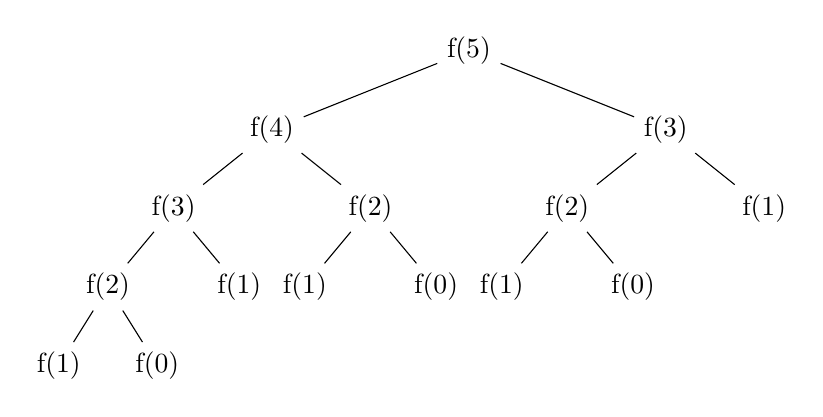
\begin{tikzpicture}[level distance=1cm,level/.style={sibling distance=5cm/(#1)}]
  \node {f(5)}
    child {node {f(4)}
      child {node {f(3)}
        child {node {f(2)}
          child {node {f(1)}}
          child {node {f(0)}}
        }
        child {node {f(1)}}
      }
      child {node {f(2)}
        child {node {f(1)}}
        child {node {f(0)}}
      }
      }
    child {node {f(3)}
      child {node {f(2)}
        child {node {f(1)}}
        child {node {f(0)}}
      }
      child {node {f(1)}
      }
    };
\end{tikzpicture}
\end{frame}

\bfr{How many times can you divide an integer in half?}

\begin{align*}
30 \rightarrow 15 \rightarrow 7 \rightarrow 3\rightarrow 1 &: 4
\\
32 \rightarrow 16 \rightarrow 8 \rightarrow 4
\rightarrow 2 \rightarrow 1 &:5
\\
40 \rightarrow 20 \rightarrow 10 \rightarrow 5
\rightarrow 2 \rightarrow 1 &:5
\\
50 \rightarrow 25 \rightarrow 12 \rightarrow 6
\rightarrow 3 \rightarrow 1 &:5
\\
64 \rightarrow 32 \rightarrow 16 \rightarrow 8 \rightarrow 4
\rightarrow 2 \rightarrow 1 &:6
\\
70 \rightarrow 35 \rightarrow 17 \rightarrow 8 \rightarrow 4
\rightarrow 2 \rightarrow 1 &:6\\
128\rightarrow 64 \rightarrow 32 \rightarrow 16 \rightarrow 8 \rightarrow 4
\rightarrow 2 \rightarrow 1 &:7\\
200\rightarrow 100 \rightarrow 50 \rightarrow 25 \rightarrow 12 \rightarrow 6
\rightarrow 3 \rightarrow 1 &:7\\
256\rightarrow 128\rightarrow 64 \rightarrow 32 \rightarrow 16 \rightarrow 8 \rightarrow 4
\rightarrow 2 \rightarrow 1 &:8
\end{align*}
\pause
\[
\lfloor\log_2(n)\rfloor \leq \log_2(n)
\]
\end{frame}

\bfr{Algorithm Analysis}
How many additions does {\tt shoop} make at a maximum?
\begin{lstlisting}
def shoop(n):
  if n == 1:
    return 7
  else:
    return shoop(n//2) + 3
\end{lstlisting}
\begin{align*}
f(1) &= 0\\
f(n) &= f(n/2) + 1\\
     &= (f(n/4) + 1) + 1\\
     &= ((f(n/8) + 1) + 1) + 1\\
     &= f(n/2^k) + k\\
     &= f(n/2^{\log_2(n)}) + \log_2(n)\\
     &= f(n/n) + \log_2(n)\\
     &= \log_2(n) = O(\log n)
\end{align*}
\end{frame}

\bfr{Algorithm Analysis}
How many additions does {\tt snarfle} make at a maximum?
\begin{lstlisting}
def snarfle(n):
  if n == 1:
    return 7
  else:
    return snarfle(n//2) + snarfle(n//2)
\end{lstlisting}
\cola
\begin{align*}
f(1) &= 0\\
f(n) &= 2f(n/2) + 1\\
     &= 2(2f(n/4) + 1) + 1\\
     &= 2^2f(n/2^2) + 2 + 1 \\
     &= 2^3f(n/2^3) + 4 + 2 + 1\\
     &= 2^kf(n/2^k) + \sum_{i=0}^{k-1}2^i 
\end{align*}
\colb\pause
\begin{align*}
     &= \ldots\\
     &= 2^{\log_2(n)}f(n/2^{\log_2(n)}) + \sum_{i=0}^{\log_2(n)-1} 2^i\\
     &= 0 + (2^{\log_2(n)-1+1}-1)/(2-1)\\
     &= 2^{\log_2(n)} - 1\\
     &= n-1 = O(n)
\end{align*}
\colc

\end{frame}


\bfr{Visualizing {\tt snarfle}}

\begin{lstlisting}
def snarfle(n):
  if n == 1:
    return 7
  else:
    return snarfle(n//2) + snarfle(n//2)
\end{lstlisting}
\[O(n)\]
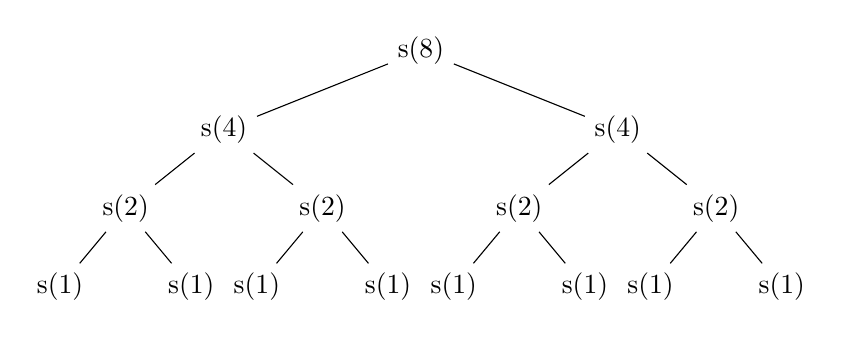
\begin{tikzpicture}[level distance=1cm,level/.style={sibling distance=5cm/(#1)}]
  \node {s(8)}
    child {node {s(4)}
      child {node {s(2)}
        child {node {s(1)}}
        child {node {s(1)}}
      }
      child {node {s(2)}
        child {node {s(1)}}
        child {node {s(1)}}
      }
      }
    child {node {s(4)}
      child {node {s(2)}
        child {node {s(1)}}
        child {node {s(1)}}
      }
      child {node {s(2)}
        child {node {s(1)}}
        child {node {s(1)}}
      }
    };
\end{tikzpicture}
\end{frame}

\bfr{What is the runtime of our multiplication algorithms?}
\cola
\bi\li Classic multiply\ei
\begin{Verbatim}[frame=single]
        238
      x  13
     ------
        714      
       238 
     ------
       3094
\end{Verbatim}

\colb
\bi \li Peasant multiply \ei
\begin{Verbatim}[frame=single]
    238   13   -->   238
    476    6
    952    3   -->   952
   1904    1   -->  1904
                    ----
                    3094
\end{Verbatim}                   
\colc

\end{frame}

\bfr{Two algorithms for {\tt power}}

$a^b = a(a^{b-1})$\hfill {\em vs.}\hfill $a^b = (a^{b/2})^2$
\begin{lstlisting}
def powlinear(a, b):
  if b == 0:
    return 1
  else:
    return a * powlinear(a, b-1)
\end{lstlisting}

\begin{lstlisting}
def powlog(a, b):
  if b == 0:
    return 1
  elif b % 2 == 1:
    return a * powlog(a, b-1)
  else:
    return powlog(a, b//2) ** 2
\end{lstlisting}

What are their running times?
\end{frame}

\bfr{Fibonacci revisited}
\begin{lstlisting}
def fibonacci(n):
  if n < 2:
    return n
  else:
    return fibonacci(n-1) + fibonacci(n-2)
\end{lstlisting}
Running time? \pause\hfill
\(O(1.7^n)\)\hfill ~
\begin{lstlisting}
def fibonacci(n):
  a,b = 0,1
  while n > 0:
    n,a,b = n-1, b, a+b
  return a
\end{lstlisting}
Runining time? \pause\hfill
\(O(n)\)
\pause
\hfill
\( 1.7^{100} > 10^{23} \gg 100 \)

\pause
Can we do better?

\end{frame}

\bfr{Fibonacci revisited}
\cola
\begin{align*}
(a,b) 
\left[\begin{array}{cc} 0 & 1 \\ 1 & 1\end{array}\right]
  &= (b, a+b)
  \\
(0,1)
\left[\begin{array}{cc} 0 & 1 \\ 1 & 1\end{array}\right]
  &= (1,1)
  \\
(0,1)
\left[\begin{array}{cc} 0 & 1 \\ 1 & 1\end{array}\right]^2
  &= (1,2)
  \\
(0,1)
\left[\begin{array}{cc} 0 & 1 \\ 1 & 1\end{array}\right]^3
  &= (2,3)
  \\
(0,1)
\left[\begin{array}{cc} 0 & 1 \\ 1 & 1\end{array}\right]^4
  &= (3,5)
  \\
(0,1)
\left[\begin{array}{cc} 0 & 1 \\ 1 & 1\end{array}\right]^5
  &= (5,8)
\end{align*}
\colb
\pause
\bi
\li Does this give you an idea?
\pause
\li Can you write a $O(\log n)$ {\tt fibonacci}?
\ei
\colc


\end{frame}

\bfr{Lab:  $O(\log n)$ {\tt fibonacci}}
\bi
\li Develop a {\tt Matrix} class that will
handle matrices of any dimension.
\li Your matrix class will handle matrix multiplication
and matrix power by overloading the \lstinline{__mul__}
and \lstinline{__pow__} methods.
\li Also develop a \lstinline{__str__} method.
\li An example interaction is at the right.
The initializing parameters for a matrix object are
the number of rows, the number of columns, and a list
of all the elements.
\li Use this class to develop a $O(\log n)$
{\tt fibonacci} function.
\li Time and compare the three fibonacci's: exponential, linear,
and log.  To get meaningful results, compare exponential and linear
in one comparison, and linear and log in another comparison.
\ei
\end{frame}
\bfr{Performance of log fibonacci}
\begin{Verbatim}[frame=single]
>>>    m = Matrix(2,2,[0,1,1,1])
>>>    for i in range(4,7):
          print(m ** i)

|    2    3|
|    3    5|

|    3    5|
|    5    8|

|    5    8|
|    8   13|
\end{Verbatim}
Time in nanoseconds for finding the 1000000th Fibonacci number:
\begin{lstlisting}
Linear: 8093750000
Log:     203125000
\end{lstlisting}
\end{frame}


\bfr{Anagram problem}
\bi
\li Determine if two strings are anagrams:

\begin{tabular}{rl}
inch & chin\\
study & dusty\\
stressed & desserts\\
cried & cider
\end{tabular}
\li
What are some algorithms?
\ei
\end{frame}

\bfr{Anagram algorithm 1: checking off}
\begin{lstlisting}
def anagramSolution1(s1,s2):
    stillOK = True
    if len(s1) != len(s2):
        stillOK = False
    alist = list(s2)
    pos1 = 0
    while pos1 < len(s1) and stillOK:
        pos2 = 0
        found = False
        while pos2 < len(alist) and not found:
            if s1[pos1] == alist[pos2]:
                found = True
            else:
                pos2 = pos2 + 1
        if found:
            alist[pos2] = None
        else:
            stillOK = False
        pos1 = pos1 + 1
    return stillOK
\end{lstlisting}
\end{frame}

\bfr{Anagram algorithm 2: sort and compare}
\begin{lstlisting}
def anagramSolution2(s1,s2):
    alist1 = list(s1)
    alist2 = list(s2)

    alist1.sort()
    alist2.sort()

    pos = 0
    matches = True

    while pos < len(s1) and matches:
        if alist1[pos]==alist2[pos]:
            pos = pos + 1
        else:
            matches = False

    return matches
\end{lstlisting}
\end{frame}


\bfr{Anagram algorithm 3: brute force}
\begin{lstlisting}
def anagramSolution3(s1, s2):
    return s1 in all_permutations(s2)

def all_permutations(s):
    if len(s) == 1:
        return [s]
    else:
        shorts = all_permutations(s[1:])
        longs = []
        for short in shorts:
            longs = longs + all_positions(s[0], short)
        return longs

def all_positions(c, s):
    strings = []
    for i in range(len(s)+1):
        strings.append(s[0:i] + c + s[i:])
    return strings
\end{lstlisting}
\end{frame}


\bfr{Anagram algorithm 4: count and compare}
\begin{lstlisting}def anagramSolution4(s1,s2):
    c1 = [0]*26
    c2 = [0]*26

    for i in range(len(s1)):
        pos = ord(s1[i])-ord('a')
        c1[pos] = c1[pos] + 1

    for i in range(len(s2)):
        pos = ord(s2[i])-ord('a')
        c2[pos] = c2[pos] + 1

    j = 0
    stillOK = True
    while j<26 and stillOK:
        if c1[j]==c2[j]:
            j = j + 1
        else:
            stillOK = False

    return stillOK
\end{lstlisting}
\end{frame}

\bfr{Runtime of Builtin Python Data Structures}

\bi
\li See text.
\ei
\end{frame}


\end{document}
